\newpage
\section{Amplificador real realimentado por tensión}
\subsection*{Introducción}
Los errores miden las desviaciones o rango de incerteza en la determinación de una medida. En el caso de los amplificadores las magnitudes involucradas son señales de tensión, corriente o sus relaciones y las desviaciones respectivas pueden ser expresadas en términos absolutos, (Ej: mV), o relativa al valor máximo que entregaría el amplificador ideal.

No obstante estos conceptos generales, cada sistema adopta modalidades particulares de expresión, por caso si el amplificador evaluado forma parte de una cadena de procesamiento de señal que termina siendo digital es atinente expresar la desviación total de aquel, en número de bits, permitiendo de esta manera coordinar adecuadamente la interfase analógica--digital.

La metodología que se utiliza para analizar y evaluar los efectos de las características reales del amplificador sobre su respuesta, consiste en ponerlos en evidencia de uno en uno idealizando las restantes. Con este procedimiento se evaluarán los errores o desviaciones respecto del comportamiento ideal del conjunto. Por razones didácticas y de uso, es de práctica usual clasificar los errores en estáticos y dinámicos. Los primeros afectan el comportamiento en continua y los segundos están relacionados fundamentalmente con la respuesta en frecuencia.
\subsection{Errores en continua}

Se puede asumir como relevantes a los producidos por las corrientes de polarización ($I_{pol}$), el desajuste de las tensiones de entrada ($V_{OS}$), la ganancia de modo diferencial finita ($A_d$) y la de modo común no nula ($A_c$).

Es necesario aclarar que la expresiones de los efectos de estas magnitudes a la salida (desviaciones) serán particulares para la los amplificadores que se toman como ejemplos, otras estructuras amplificadoras, obviamente propagaran los errores a la salida con expresiones diferentes.

\subsubsection{Efecto de las Corrientes de Polarización de Entrada (Ipol).}

Considerando que las corrientes de polarización no son nulas, la suma de corrientes en el nodo inversor, \ref{fig:2.1} resulta:

\[
i_2 - I_{pol}^- = i_1
\]

De la que se desprende que para minimizar las desviaciones debe ser:

\begin{equation}
i_2 = \frac{v_o - v^-}{R_2} >> I_{pol}^- \tag{2.1}
\end{equation}
\begin{figure}[H]
    \centering
    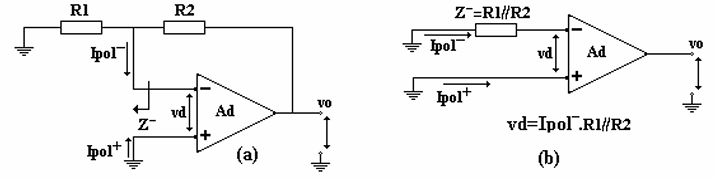
\includegraphics[width=0.5\linewidth]{Imagenes/2.1.png}
    \caption{Corrientes de polarización}
    \label{fig:2.1}
\end{figure}
Es fácil ver en esta última que el desbalance de las impedancias que cargan a ambas, se traduce en un modo diferencial de tensión a la entrada del amplificador que se puede corregir obviamente balanceando aquellas según se muestra en la \ref{fig:2.2}.
\begin{figure}[H]
    \centering
    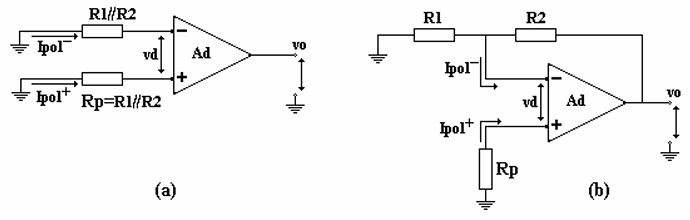
\includegraphics[width=0.5\linewidth]{Imagenes/2.2.png}
    \caption{Corrientes de polarización}
    \label{fig:2.2}
\end{figure}
\noindent La corrección mostrada arriba, anularía la desviación siempre y cuando las corrientes de polarización sean iguales, pero esto no ocurre en la realidad siendo la máxima diferencia el valor $I_{OS}$ ( desajuste de corrientes de entrada), se puede intuir entonces, que la desviación con la solución propuesta será en el peor de los casos proporcional a aquella.

\[
\Delta v_0 \propto I_{pol}^+ - I_{pol}^- = I_{os}
\]

En efecto, de Figura 11b se deduce por superposición.

\[
\Delta v_0 = \Delta v_0 \Big|_{I_{pol}^+ = 0} + \Delta v_0 \Big|_{I_{pol}^- = 0}
\]

\begin{equation} \tag{2.2}
\Delta v_0 = -I_{pol}^- \cdot R_2 + (I_{pol}^+ \cdot R_p) \cdot \left( 1 + \frac{R_2}{R_1} \right)
\end{equation}

\begin{equation} \tag{2.3}
\Delta v_0 = I_{pol}^+ \cdot R_2 - I_{pol}^- \cdot R_2 = \pm I_{os} \cdot R_2
\end{equation}

La desviación mostrada en esta última vuelve a poner en evidencia la proporcionalidad comentada entre la desviación y el valor de la resistencia de realimentación ($R_2$).l
\subsubsection{ Efecto de la Tensión de Desajuste de Entrada (VOS)}
El error producido por el desajuste de la tensión de entrada ($V_{OS}$), se puede evaluar en forma directa reduciendo su efecto a la salida a una señal de modo diferencial equivalente conectada a la entrada según se muestra en la \ref{fig:2.3}, donde el A.O. excitado por el se considera ideal.
\begin{figure}[H]
    \centering
    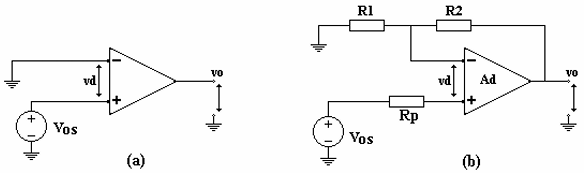
\includegraphics[width=0.5\linewidth]{Imagenes/2.3.png}
    \caption{Tensión de desajuste}
    \label{fig:2.3}
\end{figure}
\noindent En consecuencia tiene la ganancia de un configuración No Inversora Ideal.

\begin{equation} \tag{2.4}
\Delta v_0 = \pm v_{os} \left( 1 + \frac{R_2}{R_1} \right)
\end{equation}

El error total producido por los parámetros analizados, en el peor de los casos puede actuar en el mismo sentido generando un error total:

\begin{equation} \tag{2.5}
\Delta v_0 = \pm \left[ I_{os} \cdot R_2 + v_{os} \left( 1 + \frac{R_2}{R_1} \right) \right]
\end{equation}

El término que dominara en la expresión anterior, depende de la tecnología utilizada y de la calidad del amplificador. En términos generales en aquellos de tecnología (Bi-Fet) o (MOS), es mucho mas importante el producido por la tensión de offset, aunque en tecnología bipolar de precisión pueden ser muy reducido los dos.

Un problema adicional que se presenta es la dependencia de ambos parámetros con la temperatura, esto genera una deriva térmica en la tensión de salida que estará dada:

\begin{equation} \tag{2.6}
\frac{dv_0}{dT} = R_2 \cdot \frac{dI_{os}}{dT} + \frac{dv_{os}}{dT} \cdot \left( 1 + \frac{R_2}{R_1} \right)
\end{equation}

\noindent La manera típica de compensar el efecto de las corrientes de polarización es evitando que, $I_{pol}$, circule por $R_2$ excitando el nodo inversor con una fuente de corriente de igual valor. Figura 2.4, obviamente para evitar la deriva el coeficiente térmico de la corriente de compensación deberá ser igual al de la corriente de polarización, además de estar acoplada térmicamente al amplificador.
\begin{figure}[H]
    \centering
    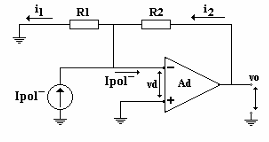
\includegraphics[width=0.5\linewidth]{Imagenes/2.4.png}
    \caption{Tensión de desajuste de entrada}
    \label{fig:2.4}
\end{figure}
\subsubsection{Efecto de la Ganancia de Lazo Abierto  (Ad, Ac)}

\noindent Se denominan de esta manera a las desviaciones de la ganancia de lazo cerrado respecto de su valor ideal, producidas por la ganancia de modo diferencial finita y de modo común no nula.

Para poner en evidencia estos errores, conocidos también como \textit{de ganancia de lazo abierto}, es necesario desarrollar las expresiones de respuesta a partir de la expresión clásica de la ganancia de lazo cerrado del amplificador realimentado (Black ).

\begin{equation} \tag{2.7}
A_{vf}(s) = \frac{A_v(s)}{1 - T(s)}
\end{equation}

\noindent $A_v(s)=$ ganancia de lazo abierto (GLA). \\
$T(s)=$ ganancia de lazo (GL).

\vspace{0.3cm}

Las expresiones anteriores de carácter general pueden ser evaluadas en el circuito de figura 2.5b, del que se deducen las siguientes relaciones particulares para la configuración no inversora.
\begin{figure}[H]
    \centering
    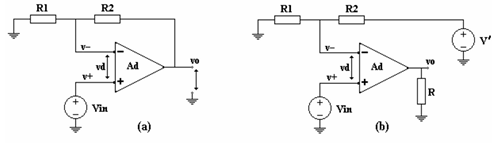
\includegraphics[width=0.5\linewidth]{Imagenes/2.5.png}
    \caption{Ganancia de lazo abierto}
    \label{fig:2.5}
\end{figure}
\noindent En efecto, considerando la ganancia de modo diferencial finita y la de modo común nula, se deduce GLA:

\begin{equation} \tag{2.8}
A_v(s) = \frac{v_0}{v_{in}} \Bigg|_{v'=0} = \frac{v_0}{v_d} \cdot \frac{v_d}{v_{in}} = A_d(s)
\end{equation}

La ganancia de bucle será:

\begin{equation} \tag{2.9}
T(s) = \frac{v_0}{v'} \Bigg|_{v_{in}=0} = \frac{v_0}{v_d} \cdot \frac{v_d}{v'} = -A_d(s) \cdot \frac{R_1}{R_1 + R_2} = -A_d(s) \cdot K
\end{equation}

En base a las relaciones expuestas del amplificador realimentado con ganancia de modo diferencial finita y a los efectos de evaluar los errores producidos, expresaremos la ganancia de lazo cerrado en una forma genérica. Así para el circuito no inversor aquella se puede expresar a partir de (1.7) de la siguiente manera:

\begin{equation} \tag{2.10}
A_{vf}(s) = \frac{A_d(s)}{1 + K \cdot A_d(s)} = \frac{1/K}{1 + \frac{1}{K \cdot A_d(s)}} = \frac{A_{vfi}}{1 - \frac{1}{T(s)}}
\end{equation}

Donde

\[
A_{vfi} = 1 + \frac{R_2}{R_1} \quad \rightarrow \quad GLC \text{ (No inversor ideal)}
\]

Expresando en los mismos términos la correspondiente a una configuración inversora, se obtiene a partir de figura 2.6
\begin{figure}[H]
    \centering
    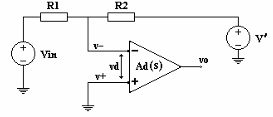
\includegraphics[width=0.5\linewidth]{Imagenes/2.6.png}
    \caption{}
    \label{fig:2.6}
\end{figure}
\noindent Ganancia de lazo abierto:

\begin{equation} \tag{2.11}
A_v(s)\big|_{v'=0} = \frac{v_0}{v_d} \cdot \frac{v_d}{v_{in}} = -A_d(s) \cdot \frac{R_2}{R_1 + R_2} = -A_d(s) \cdot (1 - K)
\end{equation}

En cambio la ganancia de lazo, (independiente del terminal en que se aplica la señal), es igual a la obtenida para la configuración no inversora.

\[
T(s)\big|_{v_{in}=0} = \frac{v_0}{v'} = -A_d(s) \cdot \frac{R_1}{R_1 + R_2} = -A_d(s) \cdot K
\]

Finalmente, GLC resulta a frecuencia cero:

\begin{equation} \tag{2.12}
A_{vf}(0) = \frac{-A_d(s) (1-k)}{1 + K \cdot A_d(s)} = \frac{ \left( 1 - \frac{1}{K} \right) }{ 1 + \frac{1}{K \cdot A_d(s)} } = \frac{A_{vfi}(0)}{1 - \frac{1}{T(0)}}
\end{equation}

El último término de (2.10) y (2.12) son formalmente iguales y se puede demostrar que otras configuraciones mostraran funciones de transferencia en lazo cerrado idénticas, además si la red de realimentación es dependiente de la frecuencia ($K(s)$) resultará la ganancia de lazo cerrado ideal también dependiente de aquella ($A_{vfi}(s)$). De manera que la expresión en cuestión puede ser asumida como alternativa general de representación de la ganancia de lazo cerrado de un amplificador realimentado, en la que además se aprecia claramente que el segundo término del denominador es el causante de la desviación del valor real de la ganancia respecto de su valor ideal. La Figura 2.7 muestra en términos de módulos, las relaciones de respuesta en frecuencia de aquella, en la que se indican los dos tipos de errores que se definen debido a la ganancia de lazo abierto finita, error de ganancia en continua $\epsilon_{G(0)}$ y dinámico $\epsilon_{G(\omega)}$.
\begin{figure}[H]
    \centering
    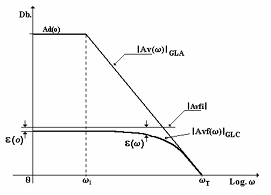
\includegraphics[width=0.5\linewidth]{Imagenes/2.7.png}
    \caption{}
    \label{fig:2.7}
\end{figure}
\noindent Ambos errores se evalúan a partir de la expresión generalizada de GLC, resultando a frecuencia cero según la expresión siguiente.

\begin{equation} \tag{2.13}
\varepsilon_{G(0)} = \frac{1}{T_0}
\end{equation}

En efecto esto se demostrará a continuación. Recordando que la ganancia de lazo ($T$) es negativa y mucho mayor que uno particularmente a frecuencia cero, se puede usar la siguiente aproximación de (2.12):

\begin{equation} \tag{2.14}
\frac{1}{1 + \varepsilon_{G(0)}} \cong 1 - \varepsilon_{G(0)}
\end{equation}

Que permite expresar aquella como:

\[
A_{vf}(0) = A_{vfi}(0) \cdot (1 - \varepsilon_{G(0)})
\]

\[
\varepsilon_{G(Ad)} = \frac{1}{T_0} = \frac{(A_{vfi}(0) - A_{vf}(0))}{A_{vfi}(0)} = \frac{\Delta A_{vf}(0)}{A_{vfi}(0)}
\]

La anterior define a $\varepsilon_{G(0)}$ , como error relativo al ideal producido por la ganancia de lazo finita, que puede ser expresado en términos absolutos según se muestra a continuación

\begin{equation} \tag{2.15}
\varepsilon_{G(Ad)} = \frac{(v_{0i} - v_{0r})}{v_{0i}} = \frac{\Delta v_0}{v_{0i}} \quad \rightarrow \quad \Delta v_0 = \varepsilon_{G(Ad)} \cdot v_{0i} \quad \text{[Volts]}
\end{equation}
\noindent De esta última se deduce, en condiciones de excitación para máxima excursión de salida (Fondo de escala, F.E), la siguiente expresión para la desviación absoluta producida por la ganancia de modo diferencial finita.

\begin{equation} \tag{2.16}
\Delta v_0 = \varepsilon_{G(Ad)} \cdot v_{0|_{\max}}
\end{equation}

Con respecto al efecto producido por la ganancia de modo común no nula, es necesario resaltar que en las configuraciones inversoras es despreciable, ya que el modo común aplicado en esta a la entrada del Amp. Op es prácticamente cero debido a que el potencial de ambas entradas es virtualmente el de tierra. En cambio por la misma razón en las configuraciones no inversoras y diferenciales en general, el modo común aplicado es el valor de la tensión en la entrada no inversora ($V^+$).

En consecuencia se analizará el error de esta última en una configuración básica. La manera clásica de ponerlo en evidencia es convertirlo en una señal de modo diferencial equivalente reducida a la entrada ($v_{ind}$), tal que amplificada por la ganancia de modo diferencial ($Ad$), produzca una tensión de salida ($v_{od}$), igual a la que produciría la de modo común ($Ac$) con la señal de modo común($v_{inc}$).

Esto es:

\begin{equation} \tag{2.17}
v_{od} = A_d \cdot v_{ind} = v_{oc} = A_c \cdot v_{inc}
\end{equation}

\noindent De la anterior se concluye que el modo diferencial equivalente vale:

\[
v_{ind} = \frac{V_{inc}}{\left( \frac{A_d}{A_c} \right)}
\]

Recordando que la relación de rechazo de modo común (RRMC) se define como la relación de las ganancias de modo diferencial y común, la anterior se puede expresar en esos términos.

\begin{equation} \tag{2.18}
v_{ind} = \frac{V_{inc}}{RRMC}
\end{equation}

A partir de esta conclusión se puede modelar al AO, exento de ganancia de modo común, Fig. 2.8, excitado por el modo diferencial equivalente.
\begin{figure}[H]
    \centering
    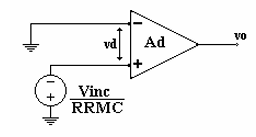
\includegraphics[width=0.5\linewidth]{Imagenes/2.8.png}
    \caption{}
    \label{fig:2.8}
\end{figure}
\noindent Si se realimenta el amplificador anterior, idealizando la ganancia de modo diferencial, que a pesar de ser un contrasentido, (haría la RRMC=$\infty$), permite poner en evidencia únicamente el efecto de la ganancia de modo común.
\begin{figure}[H]
    \centering
    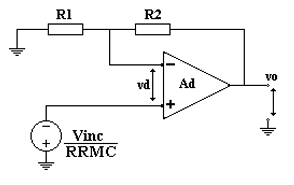
\includegraphics[width=0.5\linewidth]{Imagenes/2.9.png}
    \caption{}
    \label{fig:2.9}
\end{figure}
\noindent En efecto de la anterior se deduce para $Ad = \infty$

\begin{equation} \tag{2.19}
\Delta v_0 = \frac{v_{inc}}{RRMC} \left( 1 + \frac{R_2}{R_1} \right)
\end{equation}

\[
\Delta A_{vf} = \frac{\Delta v_0}{v_{inc}} = \frac{A_{vfi}}{RRMC}
\]

El error relativo resulta

\begin{equation} \tag{2.20}
\frac{\Delta A_{vf}(0)}{A_{vfi}(0)} = \frac{1}{RRMC} = \varepsilon_{G(Ac)}
\end{equation}

Finalmente el error producido por ambas ganancias reales a frecuencia cero es:

\begin{equation} \tag{2.21}
\varepsilon_{G(0)} = \varepsilon_{Ad} + \varepsilon_{Ac} = \frac{1}{T_0} + \frac{1}{\text{RRMC}}
\end{equation}

Cuya desviación absoluta es:

\begin{equation} \tag{2.22}
\Delta v_0 = \varepsilon_{Ad0} \cdot v_{0\text{max}} + \varepsilon_{Ac0} \cdot v_{inc} \cdot A_{vfiN}
\end{equation}

Ambos términos de error expresados en la anterior pueden ser del mismo orden de magnitud, además presentan una significativa dispersión y dependencia con la temperatura. Esta desviación adicional puede ser evaluada en el caso de la ganancia de modo diferencial, a partir de la función sensitividad cuya expresión para grandes variaciones está aproximada en las siguientes expresiones.

\begin{equation} \tag{2.23}
S_{A_d(0)}^{A_{vf}(0)} = \frac{\frac{\Delta A_{vf}(0)}{A_{vf}(0)}}{\frac{\Delta A_d(0)}{A_d(0)}} \cong \frac{1}{1 + K \cdot A_d(0) + K \cdot \Delta A_d(0)}
\end{equation}

El error relativo adicional deducido de está será:

\begin{equation} \tag{2.24}
\varepsilon_0 (\Delta A_d) = \frac{\Delta A_d(0)}{A_d(0)} \cdot S_{A_d(0)}^{A_{vf}(0)} = \frac{\Delta A_d(0)}{A_d(0)} \cdot \left( \frac{1}{1 + K \cdot A_d(0) + K \cdot \Delta A_d(0)} \right)
\end{equation}
\subsubsection{Integración de errores}
\noindent Las desviaciones evaluadas, en el peor de los casos, afectan la salida en el mismo sentido y la desviación total ($\Delta v_{0T}$), puede ser expresada según se comentó, en voltios o en términos relativos al fondo de escala o en número de bits. En este último caso se compara al número de bits que requeriría un conversor A/D, para discriminar dentro del fondo de escala un nivel de tensión equivalente a la desviación total.

\begin{equation}
\Delta v_{0T} \leq \frac{V_{FE}}{2^n}
\end{equation}
\subsection{Respuesta en frecuencia}
\noindent La disminución de la ganancia de lazo abierto con la frecuencia, debido a la presencia de los polos del amplificador básico, adicionan errores que se denominan genéricamente dinámicos. Debido a que la definición y cuantificación de los mismos se efectúa a partir de la respuesta en frecuencia en lazo cerrado de la configuración, es necesario previamente analizar aquella en las configuraciones simples, donde se definirán conceptos y relaciones útiles para tratar formalmente los errores dinámicos relevantes. Se considerará al amplificador básico con ganancia de modo diferencial con un solo polo en la banda de utilización (2.26) y red de realimentación resistiva pura.

\begin{equation} \tag{2.26}
A_d(s) = \frac{A_d(0)}{\left( 1 + \frac{s}{\omega_1} \right)}
\end{equation}

A partir de formula de Black se deduce para la configuración no inversora, la siguiente expresión de GLC.

\begin{equation} \tag{2.27}
A_{vf}(0) = \left[ \frac{A_d(0)}{1 + K.A_d(0)} \right] \cdot \left[ \frac{1}{1 + \frac{s}{\omega_1.(1+K.A_d(0))}} \right] = \frac{A_{vf}(0)}{\left( 1 + \frac{s}{\omega_H} \right)}
\end{equation}

Donde el ancho de banda de 3db está dado por la siguiente expresión:

\begin{equation} \tag{2.28}
\omega_H = \omega_1.(1-T_0) \cong \omega_1.k.A_d(0)
\end{equation}

Tal que el producto ganancia ancho de banda resulta constante:

\begin{equation} \tag{2.29}
GBW = A_{vf}(0).\omega_H = A_d(0).\omega_1 = \omega_T
\end{equation}

La frecuencia de cruce por cero, ($\omega_T$), es un parámetro relevante para la selección del amplificador y es muy útil para la síntesis del mismo, relacionarlo con los requerimientos de ancho de banda y cantidad de realimentación del amplificador realimentado

\begin{equation} \tag{2.30}
\omega_H \cong \omega_1.k A_d(0) = \omega_T.k
\end{equation}

Las magnitudes involucradas en las expresiones anteriores se muestran en el diagrama de módulos de la Figura 2.9
\begin{figure}[H]
    \centering
    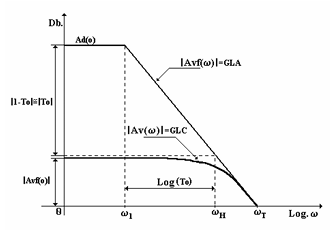
\includegraphics[width=0.5\linewidth]{Imagenes/2.10.png}
    \caption{}
    \label{fig:2.12}
\end{figure}
\noindent Repitiendo el análisis para la configuración inversora, se obtiene:

\begin{equation} \tag{2.31}
A_{vf}(s) = \frac{-A_d(s).(1-K)}{1 + K.A_d(s)} = \frac{-A_d(0).(1-K)}{1 + K.A_d(0)} \cdot \frac{1}{1 + \frac{s}{\omega_1.(1 + K.A_d(0))}}
\end{equation}

\begin{equation} \tag{2.32}
A_{vf}(s) = \frac{A_{vf}(0)}{\left( 1 + \frac{s}{\omega_H} \right)}
\end{equation}

\noindent Donde la ganancia en la banda de paso y el ancho de banda están dados por las siguientes expresiones respectivas

\begin{equation} \tag{2.33}
A_{vf}(0) = \frac{-A_d(0).(1-K)}{1 - T_0}
\end{equation}

\begin{equation} \tag{2.34}
\omega_H \cong \omega_1.k.A_d(0) = \omega_T.k
\end{equation}

\noindent Debe notarse que (2.34), repite la expresión del caso no inversor transformándose en general para amplificadores realimentados con $K$ real y función de transferencia del amplificador con un solo polo.
\begin{figure}[H]
    \centering
    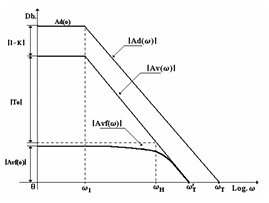
\includegraphics[width=0.5\linewidth]{Imagenes/2.11.png}
    \caption{}
    \label{fig:2.11}
\end{figure}
\noindent A partir de (2.34) debe notarse que la frecuencia de corte de 3 db, ($\omega_H$) será la misma para diferentes configuraciones siempre que tengan idéntica cantidad de realimentación, pero esto implica diferentes ganancias de lazo cerrado ($A_{vfi}=f(K)$), por caso, para los ejemplos analizados NI e IN resultaron:

\[
A_{vfi (NI)} = \frac{1}{K} \quad \text{y} \quad A_{vfi (Inv)} = - \frac{1-K}{K}
\]
Los siguientes ejemplos ilustran el tema.

\noindent \textbf{\large Ejemplo 2.1}

\vspace{0.2cm}

\noindent Demostrar que, si se implementa una configuración NI e IN, de ganancia ideal unitaria, utilizando un A.O con F de T, de un solo polo y frecuencia de cruce $\omega_T$, el inversor tiene la mitad de ancho de banda que el primero.

\vspace{0.3cm}
\hrule
\vspace{0.3cm}

\noindent En efecto:

\[
A_{vfi}\Big|_{NI} = 1 = \frac{1}{K} \Rightarrow k=1 \Rightarrow \omega_H = K.\omega_T = \omega_T
\]

\noindent En cambio para la misma ganancia en configuración inversora será :

\[
A_{vfi}\Big|_{Inv} = -1 = 1 - \frac{1}{K} \Rightarrow K = \frac{1}{2} \Rightarrow \omega_H = \frac{1}{2}.\omega_T
\]

\vspace{0.3cm}
\hrule
\vspace{0.3cm}

\noindent \textbf{\large Ejemplo 2.2}

\vspace{0.2cm}

\noindent A partir del gráfico de fig E.2.2, demostrar que la relación entre las frecuencias de cruce de la ganancia de lazo abierto NI e IN es

\[
\omega'_T = \omega_T.(1-K)
\]

\vspace{0.3cm}
\hrule
\begin{figure}[H]
    \centering
    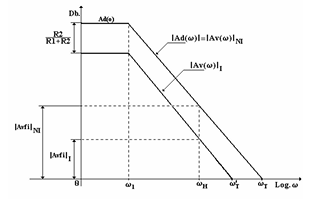
\includegraphics[width=0.5\linewidth]{Imagenes/2.12.png}
    \caption{}
    \label{fig:2.12}
\end{figure}
\noindent \textbf{\large Ejemplo 2.3}

\vspace{0.2cm}

\noindent Analizar la respuesta en frecuencia del amplificador logarítmico.

\vspace{0.3cm}
\hrule
\vspace{0.3cm}

\noindent Es útil analizar la respuesta en frecuencia de aplicaciones amplificadoras realimentadas activamente como lo es por ejemplo el amplificador logarítmico (sección 1.2), debido a que en este caso la ganancia de lazo en continua ($T_0$), puede exceder largamente la de lazo abierto del amplificador básico debido al aporte adicional puesto en el lazo, por el amplificador base común que lo realimenta. Resultando en consecuencia la ganancia de lazo cerrado menor que uno, como se aprecia en el diagrama de módulos E.2.13.

\[
\big| A_{vf}(\omega) \big|_{dB} = \big| GLA(\omega) \big|_{dB} - \big| T(\omega) \big|_{dB}
\]

\noindent En efecto la figura E.2.3.1 muestra al amplificador con el lazo abierto y el transistor reemplazado por su circuito lineal equivalente de baja frecuencia para la conexión base común, del que se deducen las siguientes expresiones.
\begin{figure}[H]
    \centering
    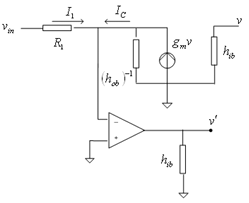
\includegraphics[width=0.5\linewidth]{Imagenes/2.13.png}
    \caption{}
    \label{fig:2.13}
\end{figure}
\[
GLA\big|_{V=0} = - \left( \frac{h_{ob}^{-1}}{R_1 + h_{ob}^{-1}} \right) . A_d(s) \cong A_d(s)
\]

\[
K\big|_{V_{in}=0} = \frac{v'}{v} = gm.R_1
\]

\[
T(s) = \frac{v'}{v} = K.GLA = \frac{-gm.R_1.A_d(0)}{ \left( 1 + \frac{s}{\omega_1} \right) }
\]

\noindent Recordando que: $gm = I_C/V_T$, la ganancia de lazo será proporcional a la corriente de colector y a través de esta de la tensión de entrada, ($I_C=V_{in}/R_1$), tal que a frecuencia cero resulta:

\[
T(0) = - \left( \frac{I_C}{V_t} \right) .R_1.A_d(0) = - \frac{V_{in}}{V_t} . A_d(0) = -K_0 . A_d(0)
\]

\noindent Tomando como ejemplo el VFA OPA627, cuyos datos relevantes son:

\[
A_d(0) = 116dB; \quad f_T = 16MHz \quad \text{y} \quad f_1 = 25Hz
\]

\noindent Para la tensión máxima de señal (10 V), la ganancia de lazo resulta aproximadamente

\[
T(0) = 168 \ dB \Rightarrow \Big| A_{vf}(0) \Big| = -52 \ dB
\]

\noindent Esta dependencia directa de la ganancia de lazo con la amplitud de la señal de entrada, se traslada también al ancho de banda.
\begin{figure}[H]
    \centering
    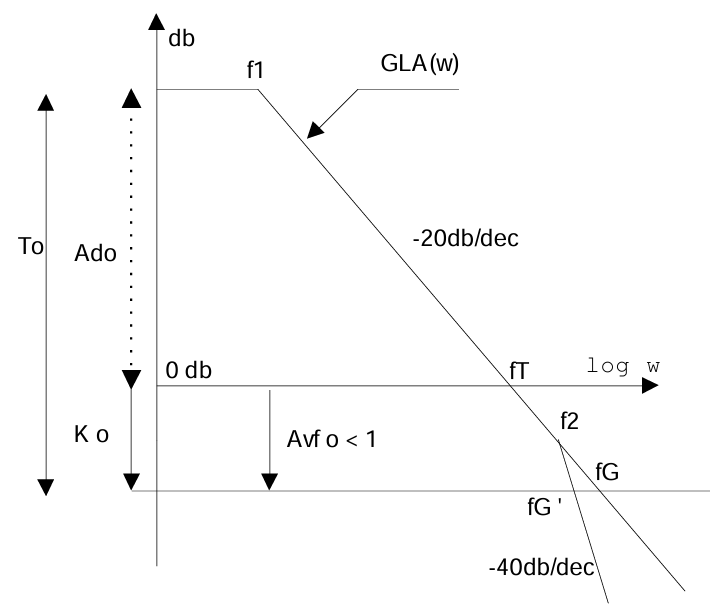
\includegraphics[width=0.5\linewidth]{Imagenes/2.14.png}
    \caption{}
    \label{fig:2.14}
\end{figure}

\[
\omega_H = K.\omega_T = \frac{V_{in}}{V_t}.\omega_T
\]

\noindent Resultando

\noindent $\omega_H = \omega_T$ para $V_{in} = V_t$ y $\omega_H > \omega_T$ para $V_{in} > V_t$

\vspace{0.3cm}

\noindent La dependencia del ancho de banda con la amplitud de la señal, es un problema en este tipo de amplificador, que se agrava sensiblemente si se tiene en cuenta que este generalmente presenta un segundo polo dentro de la década siguiente a la frecuencia de cruce (como muestra en línea de puntos la figuras E.2.3.2), tal que si la frecuencia a que la ganancia de lazo se hace unitaria ($f_{G'}$), es mayor que aquella, el amplificador se tornará inestable.

\vspace{0.5cm}
\hrule
\vspace{0.2cm}

\noindent \textbf{\large Ejemplo 2.4}

\vspace{0.2cm}

\noindent Demostrar que la frecuencia de corte del amplificador diferencial de Fig. 1.6, (Sección 1.1), responde a la expresión dada por (2.34).

\vspace{0.3cm}
\hrule
\vspace{0.3cm}

\noindent Considerando al amplificador con función de transferencia de un solo polo, $A_d(s) = \frac{A_d(0)}{\left( 1 + \frac{s}{\omega_1} \right)}$ y a partir de la expresión de Black, se calculará la ganancia de lazo cerrado desde el circuito siguiente.
\begin{figure}[H]
    \centering
    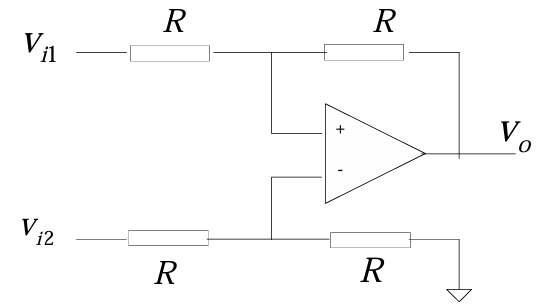
\includegraphics[width=0.5\linewidth]{Imagenes/2.15.png}
    \caption{}
    \label{fig:2.15}
\end{figure}
La ganancia de lazo abierto de cada una de las señales de excitación es:

\[
GLA_1 = \left. \frac{v_o}{v_{i1}} \right|_{v_{i2}=v'=0} = - \frac{R}{R+R} A_d(s) \qquad \text{y} \qquad GLA_2 = \left. \frac{v_o}{v_{i2}} \right|_{v_{i1}=v'=0} = \frac{R}{R+R} A_d(s)
\]

Luego la ganancia de lazo abierto global es:

\[
GLA_1 + GLA_2 = \left. \frac{v_o}{v_{i2} - v_{i1}} \right|_{v,v'=0} = \frac{R}{R+R} . A_d(s)
\]

La ganancia de lazo resulta;

\[
\text{T} = \left. \frac{v_o}{v_i'} \right|_{v_{i1}=v_{i2}=v'=0} = - \frac{R}{R+R} A_d(s) = -k . A_d(s)
\]

Finalmente se resuelve la de lazo cerrado.

\begin{equation}
GLC = \frac{v_o}{v_{i2} - v_{i1}} = \frac{k.A_d(s)}{1 + k.A_d(s)} = \frac{\frac{k.A_d(0)}{(1+s/\omega_1)}}{1 + \frac{k.A_d(0)}{(1+s/\omega_1)}} = \frac{A_{vf}(0)^{Dif1}}{\left( 1 + \frac{s}{\omega_1 . A_d(0) . k} \right)} = \frac{A_{vf}(0)^{Dif1}}{\left( 1 + \frac{s}{\omega_{H1}} \right)} \tag{E.2.4.1}
\end{equation}

En la anterior es

\begin{equation}
A_{vf}(0) = \frac{k.A_d(0)}{1 + k.A_d(0)} \cong \frac{R}{R} = 1 \qquad \text{y} \qquad f_{H1} = k . f_T = \frac{1}{2} f_T = 8 \text{ MHz} \tag{E.2.4.2}
\end{equation}
\hrule
\vspace{1.5mm}
\noindent \textbf{Ejemplo 2.5}
\vspace{1.5mm}
\hrule
\vspace{4mm}
\noindent Calcular el ancho de banda del amplificador del problema 1.3 con los valores dados en el circuito siguiente y utilizando el mismo amplificador VFA que en el ejemplo anterior.
\vspace{4mm}
\hrule
\begin{figure}[H]
    \centering
    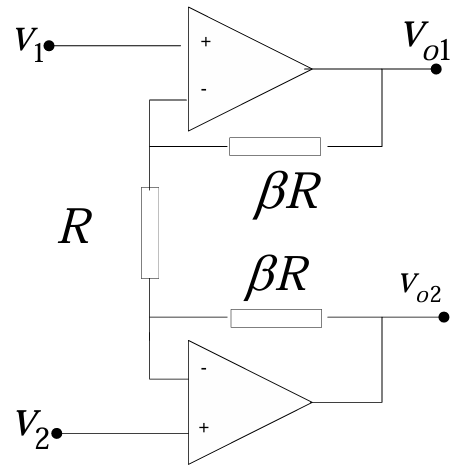
\includegraphics[width=0.5\linewidth]{Imagenes/2.16.png}
    \caption{}
    \label{fig:2.16}
\end{figure}
\noindent Utilizando superposición se deduce por inspección que la salida $v_{01}$ estará conformada por el aporte de $v_1$ con la ganancia no inversora dada por (2.27) y el de $v_2$ con la inversora dada por (2.32).

\[
v_{01} = \left( \frac{A_{vf}(0)^{NI}}{1 + \frac{s}{\omega_{H2}}} \right) v_1 + \left( \frac{A_{vf}(0)^{In}}{1 + \frac{s}{\omega_{H2}}} \right) v_2
\]

\vspace{0.8cm}

\[
v_{02} = \left( \frac{A_{vf}(0)^{NI}}{1 + \frac{s}{\omega_{H2}}} \right) v_2 + \left( \frac{A_{vf}(0)^{In}}{1 + \frac{s}{\omega_{H2}}} \right) v_1
\]

\vspace{0.3cm}

\noindent Con \quad $\omega_{H2} = \omega_1 . A_d(0) . k = \omega_T . k \quad$ y $\quad k = \frac{R}{R + \beta . R} = \frac{1}{1 + \beta}$ \hfill (E.2.51)

\vspace{0.5cm}

\noindent De las anteriores se deduce la ganancia de modo diferencial.

\begin{equation} \tag{E.2.5.2}
v_{02} - v_{01} = \left( \frac{v_2 - v_1}{1 + \frac{s}{\omega_{H2}}} \right) (A_{vf}(0)^{Dif2}) \quad \Rightarrow \quad \frac{v_{02} - v_{01}}{v_2 - v_1} = \frac{A_{vf}(0)^{Dif2}}{1 + \frac{s}{\omega_{H2}}}
\end{equation}

\vspace{0.5cm}

\noindent Finalmente \quad $\omega_{H2} = \left( \frac{1}{11} \right) . \omega_T = 0,09 . \omega_T$
\noindent \textbf{\large Ejemplo 2.6}

\vspace{0.2cm}

\noindent Analizar la respuesta en frecuencia del amplificador que resulta de conectar en cascada el amplificador diferencial del ejemplo 2.4 con el respectivo del ejemplo 2.5, configurando lo que se denomina amplificador de instrumentación.

\vspace{0.4cm}

\noindent En efecto a partir de (E.2.5.2) y (E.2.4.1) se deduce:

\begin{equation*}
\left( \frac{v_{02} - v_{01}}{v_2 - v_1} \right) \cdot \left( \frac{v_0}{v_{02} - v_{01}} \right) = \frac{A_{vf}(0)^{Dif1} \cdot A_{vf}(0)^{Dif2}}{ \left( 1 + \frac{s}{\omega_{H1}} \right) \left( 1 + \frac{s}{\omega_{H2}} \right) }
\end{equation*}

\vspace{0.4cm}

\noindent La anterior muestra una función de transferencia de dos polos, con una separación entre dos y tres octavas. Una primera aproximación manual a la frecuencia de corte de la cascada sería por polo dominante, ($\omega_H \cong \omega_{H1}$) o por suma de las constantes de tiempo respectivas.
\subsubsection{Respuesta en frecuencia}
\noindent Asumiendo el carácter complejo de la GLC dado por cualquiera de sus expresiones matemáticas, se pone en evidencia que los errores a tratar están relacionados con el módulo y fase respectivos o con ambos simultáneamente. Denominándose los dos primeros como de ganancia o \textit{distorsión de frecuencia}, y de fase o \textit{distorsión de retardo} respectivamente.

\begin{equation} \tag{2.35}
A_{vf}(\omega) = \big| A_{vf}(\omega) \big| e^{j \arg(A_{vf}(\omega))}
\end{equation}

\noindent En referencia a la figura 2.12 y asumiendo el carácter de las magnitudes involucradas, se interpreta el error dinámico en términos generales como la diferencia de la tensión de salida ideal y la real a una frecuencia determinada del amplificador realimentado.

\[
\Delta \bar{V}_o = \bar{V}_{oi} - \bar{V}_{o\omega}
\]

\noindent La anterior se expresa en términos relativos, según la siguiente

\begin{equation} \tag{2.36}
\bar{\varepsilon}_\omega = \frac{\Delta \bar{V}_o}{\bar{V}_{oi}} = \frac{\bar{A}_{vfi} - \bar{A}_{vf}(\omega)}{\bar{A}_{vfi}}
\end{equation}

\noindent Teniendo presente la expresión genérica de GLC, (2.12), la (2.36) puede ser expresada de manera compacta

\begin{equation} \tag{2.37}
\bar{\varepsilon}_\omega = \frac{\Delta \bar{V}_o}{\bar{V}_{oi}} = 1 - \frac{\bar{A}_{vf}(\omega)}{\bar{A}_{vfi}} = 1 - \bar{a}_{f(\omega)} = 1 - \frac{1}{1 - \frac{1}{T(\omega)}}
\end{equation}
\begin{figure}[H]
    \centering
    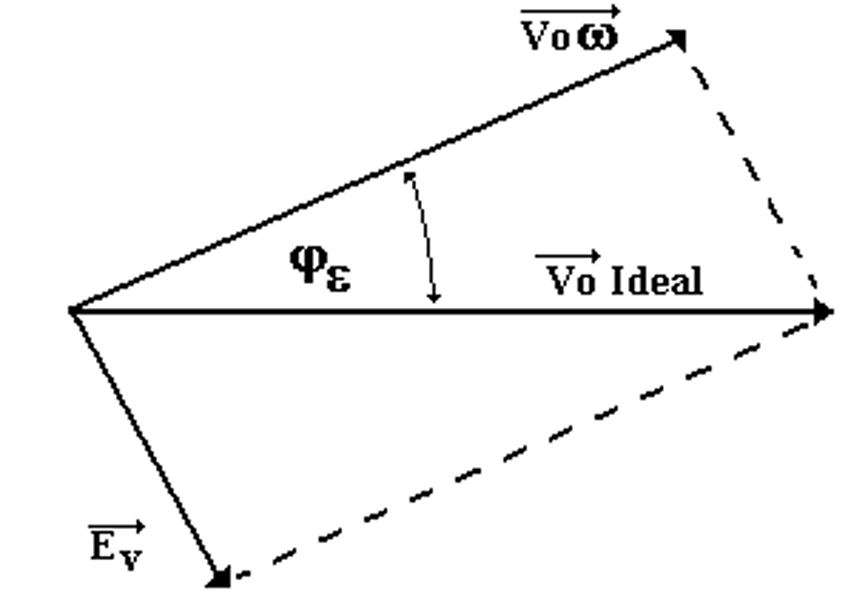
\includegraphics[width=0.5\linewidth]{Imagenes/2.17.png}
    \caption{Enter Caption}
    \label{fig:placeholder}
\end{figure}
\subsubsection{Error vectorial ($\boldsymbol{\varepsilon}_v$)}
\noindent A partir de la ecuación (2.37) se define el error vectorial como el módulo de la diferencia expresada por esta.

\begin{equation} \tag{2.38}
\varepsilon_v = \left| 1 - \frac{1}{1 - \frac{1}{T(\omega)}} \right|
\end{equation}

\noindent Se debe notar que el error vectorial puede ser significativo aun cuando los módulos respectivos no lo sean. La anterior puede expresarse de manera muy simple utilizando la aproximación (2. 14)

\begin{equation} \tag{2.39}
\varepsilon_v = \left| 1 - \frac{1}{1 - \frac{1}{T(\omega)}} \right| = \left| 1 - \left( 1 + \frac{1}{T(\omega)} \right) \right| \cong \left| \frac{1}{T(\omega)} \right|
\end{equation}

\noindent Para \quad $\big| T(\omega) \big| \gg 1$

\vspace{0.3cm}

\noindent Según la anterior el error vectorial puede leerse en decibeles desde el diagrama de módulos de fig 2.13, teniendo presente que son negativos, como corresponde cuando el argumento del logaritmo es menor que uno

\[
\varepsilon_v \big|_{dB} = 1\big|_{dB} - \big| T(\omega) \big|_{dB}
\]

\vspace{0.3cm}

\noindent La expresión (2.39) puede relacionarse con el ancho de banda de 3db ($\omega_H$) y el producto GBW del amplificador, arrojando una ecuación muy práctica para el cálculo manual.

\noindent En efecto teniendo presente que la ganancia de lazo es

\[
T(s) = -k.A_d(s) = \frac{-k.A_d(0)}{\left( 1 + \frac{s}{\omega_1} \right)}
\]

\noindent Se deduce

\begin{equation} \tag{2.40}
\varepsilon_v \cong \left| \frac{1}{T(\omega)} \right| = \left| \frac{1 + j(\omega / \omega_1)}{k.A_d(0)} \right| \cong \frac{1}{T(0)} \cdot \frac{\omega}{\omega_1} = \frac{\omega}{k.A_d(0).\omega_1} = \frac{\omega}{k.\omega_T} = \frac{\omega}{\omega_H}
\end{equation}

\noindent Para $\omega_H \gg \omega$
\begin{figure}[H]
    \centering
    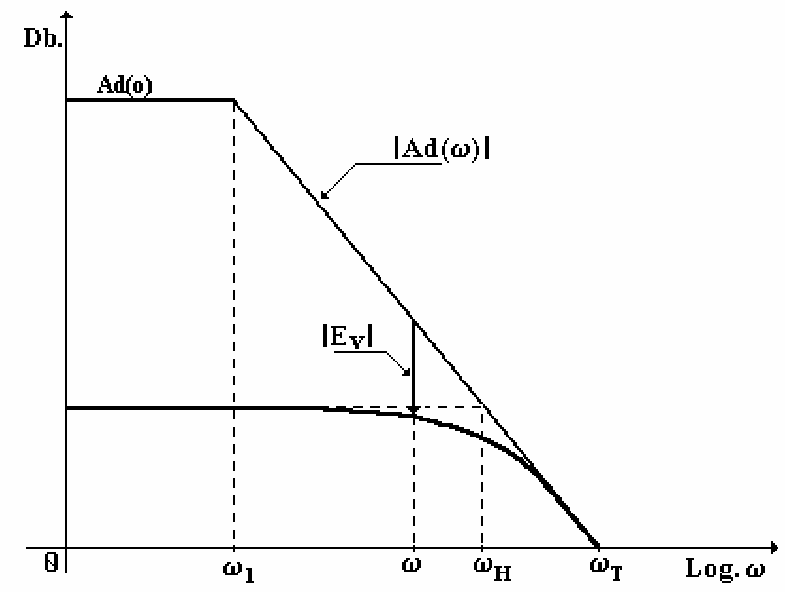
\includegraphics[width=0.5\linewidth]{Imagenes/2.18.png}
    \caption{}
    \label{fig:2.18}
\end{figure}
\subsubsection{Error de Ganancia ($\varepsilon_G(\omega)$)}
\noindent Definido también por \textit{distorsión de frecuencia}, involucra la diferencia de los módulos de los vectores expresados en la ecuación (2.37)

\begin{equation}
    \varepsilon_G = 1 - \left| \frac{1}{1 - \dfrac{1}{T(\omega)}} \right| \cong 1 - \left| 1 + \frac{1}{T(\omega)} \right| \approx 1 - \sqrt{1 + \left( \frac{\omega}{\omega_H} \right)^2} \tag{2.41}
\end{equation}

\vspace{2mm}
\noindent $T(\omega) \gg 1$
\vspace{4mm}

\noindent Al igual que en el caso del error vectorial la anterior puede llevarse a una forma más sencilla utilizando la siguiente aproximación serial para el modulo expresado en ella.

\begin{equation}
    \sqrt{1 + x} \approx 1 + \frac{x}{2} \tag{2.42}
\end{equation}

\noindent $x \ll 1$
\vspace{4mm}

\noindent La (2.41) queda expresada por

\begin{equation}
    \varepsilon_G \cong \frac{1}{2} \left( \frac{\omega}{\omega_H} \right)^2 \tag{2.43}
\end{equation}

\noindent $\omega_H \gg \omega$
\vspace{4mm}

\noindent La manera frecuente de expresar el error de ganancia es como lo muestra la siguiente

\begin{equation}
    (\varepsilon_G)_{Db} = |A_{vfl}|_{Db} - |A_{vf}(\omega)|_{Db} \tag{2.44}
\end{equation}
\noindent De la que se deriva la siguiente

\begin{equation}
|\varepsilon_G|_{Db} = 20 \cdot \log \left( \frac{|A_{vfl}|}{|A_{vf}(\omega)|} \right) \tag{2.45}
\end{equation}

\noindent En esta definición el error evaluado a la frecuencia del codo del diagrama asintótico (Fig. 2.13) es:

\begin{equation*}
\varepsilon_G \big|_{\omega_H} = 3 \text{ dB}
\end{equation*}

\noindent Es de mucha utilidad para el diseño, relacionar el error de ganancia expresado según (2.45) con el producto GBW del amplificador y la ganancia de lazo cerrado ideal.

\noindent Asumiendo que a las frecuencias del extremo superior de la banda se puede considerar:

\begin{equation}
A_{vf(0)} \cong A_{vfl} \tag{2.46}
\end{equation}

\noindent Esto equivale despreciar el error producido por la ganancia no ideal a frecuencia cero. La expresión (2.27), se puede expresar según (2.47).

\begin{equation}
A_{vf}(\omega) = \frac{A_{vf}(0)}{1 + j \dfrac{\omega}{\omega_H}} \cong \frac{A_{vfl}}{1 + j \dfrac{\omega}{\omega_H}} \tag{2.47}
\end{equation}

\noindent La relación de módulos es a partir de esta última.

\begin{equation}
\left| \frac{A_{vfl}}{A_{vf}(\omega)} \right| = \sqrt{1 + \left( \frac{\omega}{\omega_H} \right)^2} \tag{2.48}
\end{equation}

\noindent Además el error dado por (2.45), puede expresarse como:

\begin{equation}
\left| \frac{A_{vf}(\omega)}{A_{vfl}} \right| = 10^{-\frac{\varepsilon_G}{20}} \tag{2.49}
\end{equation}

\noindent Relacionando las anteriores se obtiene finalmente la siguiente:

\begin{equation}
\omega = \omega_H \cdot \sqrt{10^{\frac{\varepsilon_G}{10}} - 1} = K \cdot \omega_T \cdot \sqrt{10^{\frac{\varepsilon_G}{10}} - 1} \tag{2.50}
\end{equation}

\noindent Esta última expresión es muy útil en el proceso de síntesis ya que permite coordinar la ganancia de lazo cerrado ideal, $f(k)$, con el amplificador a utilizar $(\omega_T)$ y la distorsión de frecuencia requerida en $dB, (\varepsilon_G)$, a una frecuencia dada $(\omega)$.
\subsubsection{Errores en la Respuesta para Señales Fuertes}
Es necesario para la comprensión del problema remitirse, aunque con todas las simplificaciones 
posibles, a la estructura interna del amplificador. Por ejemplo el mostrado en Figura 2.14, que re
presenta un caso típico de amplificador VFA. La  primer etapa en configuración diferencial puede 
ser modelada por una fuente de corriente controlada por el modo diferencial de entrada de muy alta 
impedancia de salida (OTA), infinita para el caso, cargada por una de emisor común (Q5 y Q6) de 
muy alta ganancia cuya salida finalmente excita un amplificador separador de ganancia de tensión 
unitaria(Simetría Complementaria).
\begin{figure}[H]
    \centering
    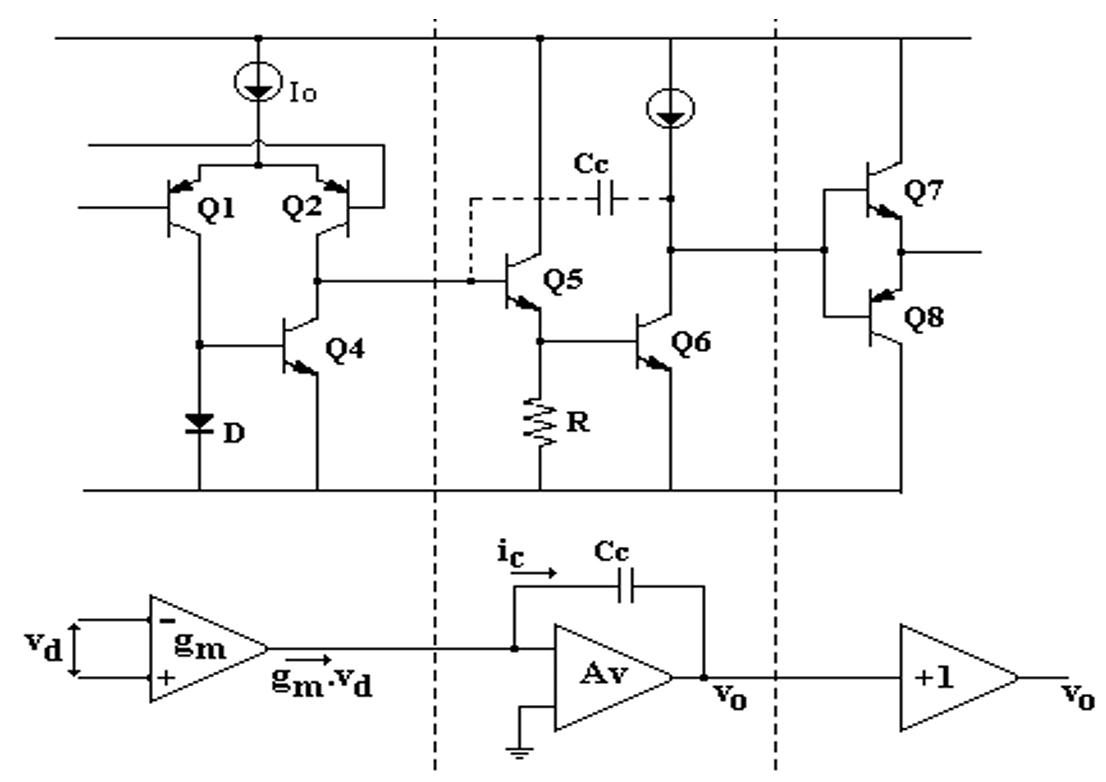
\includegraphics[width=0.5\linewidth]{Imagenes/2.19.png}
    \caption{}
    \label{fig:2.19}
\end{figure}
El amplificador descrito, sin el capacitor Cc conectado, tiene típicamente una función de transferen
cia, para el modo diferencial de entrada con tres polos en la banda de utilización (Fig 2.15).
\begin{figure}[H]
    \centering
    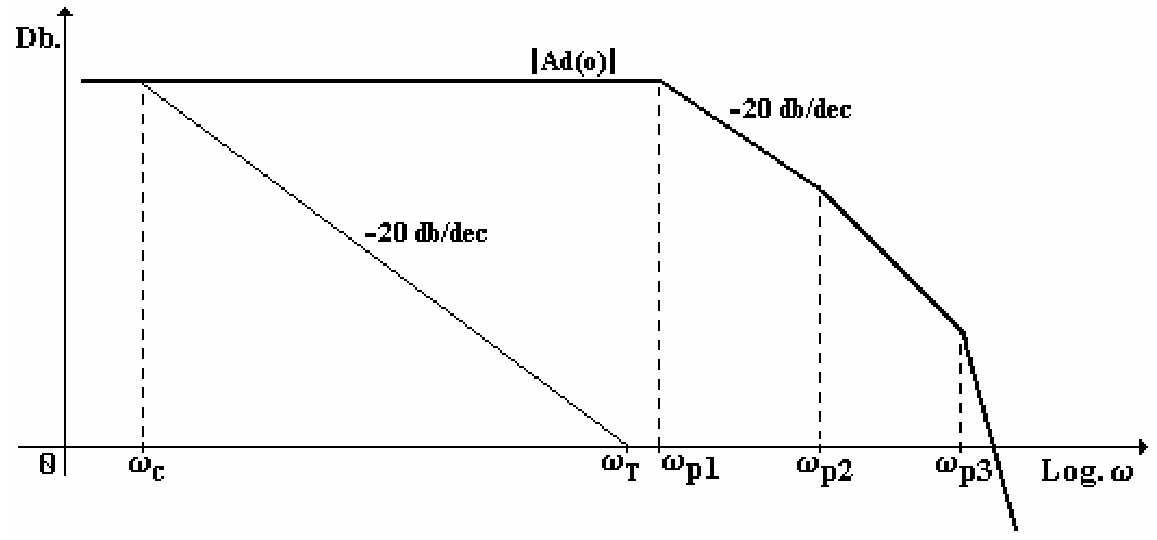
\includegraphics[width=0.5\linewidth]{Imagenes/2.20.png}
    \caption{}
    \label{fig:2.20}
\end{figure}
\noindent Si a un amplificador con este tipo de respuesta se lo realimenta suficientemente presentará problemas de estabilidad. Debido a que en aplicaciones de continua o no muy altas frecuencias, no se requiere un ancho de banda apreciable, el fabricante modifica la característica de respuesta, integrando el capacitor $C_C$ (generalmente de un valor alrededor de los 30pf), a los efectos de generar un polo dominante, ($\omega_C$ en Figura 2.15), en la función de transferencia, tal que el primer polo de la función original ($\omega_{p1}$), quede fuera de la banda de utilización ($\omega_{p1} > \omega_T$). Esta modificación de la respuesta, si bien elimina los potenciales problemas de estabilidad, reduce drásticamente la banda de utilización del mismo para señal débil, hecho que se agrava cuando el amplificador ha de trabajar con grandes excursiones de la tensión de salida. Este último efecto se analizará a continuación.
\begin{figure}[H]
    \centering
    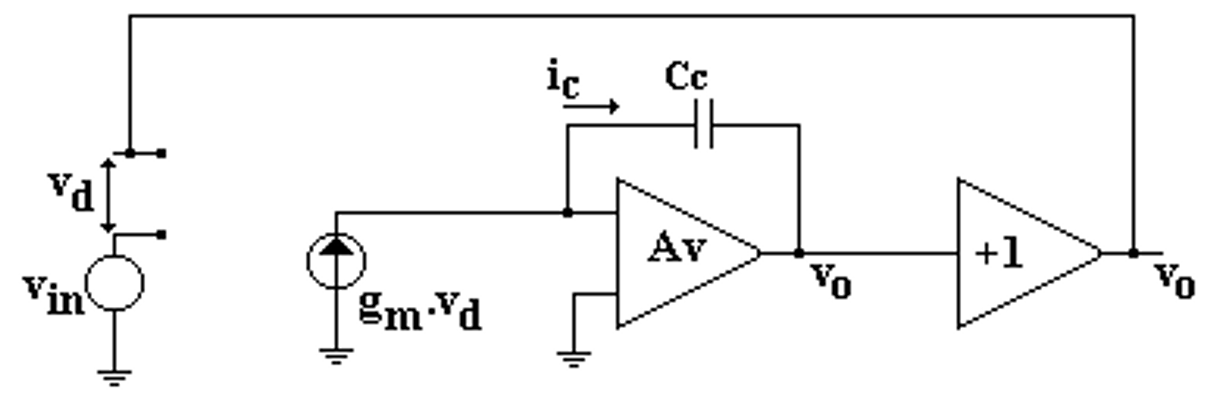
\includegraphics[width=0.5\linewidth]{Imagenes/2.21.png}
    \caption{}
    \label{fig:2.21}
\end{figure}
\noindent Si el amplificador internamente compensado se realimenta negativamente configurando por ejemplo, uno de ganancia unitaria (Buffer). Figura 2.16, se obtiene

\begin{equation} \tag{2.51}
v_0 = v_C
\end{equation}

Y la velocidad de crecimiento de la tensión de salida es

\begin{equation} \tag{2.52}
\frac{dv_0}{dt} = \frac{dv_C}{dt}
\end{equation}

La expresión anterior puede ser puesta en términos de la corriente de señal

\[
C_C \cdot \frac{dv_0}{dt} = C_C \cdot \frac{dv_C}{dt} = i_c = g_m \cdot v_d
\]

Luego

\begin{equation} \tag{2.53}
\frac{dv_0}{dt} = \frac{1}{C_C} \cdot g_m \cdot v_d
\end{equation}

\noindent La anterior muestra que la velocidad de crecimiento de la tensión de salida es proporcional a la corriente de señal disponible a la salida del diferencial, ($g_m \cdot v_d$) y esta tiene como cota superior a la correspondiente a la de polarización de esa etapa ($I_o$), evento que se alcanza cuando el modo diferencial de entrada es cercano al máximo ($v_d \text{ máx}$).

\vspace{0.3cm}

\noindent Se debe recordar que este último es de aproximadamente 100 mV para una etapa diferencial bipolar clásica y del orden del volt, para una de tecnología de efecto de campo.

\vspace{0.3cm}

\noindent Ahora bien, si en el ejemplo que se analiza la señal es débil ($v_{in} \ll v_{d \text{ máx}}$ ), a pesar del retraso de la salida respecto de la entrada (fig. 2.17a) aquella copia la entrada (operación lineal).
\begin{figure}[H]
    \centering
    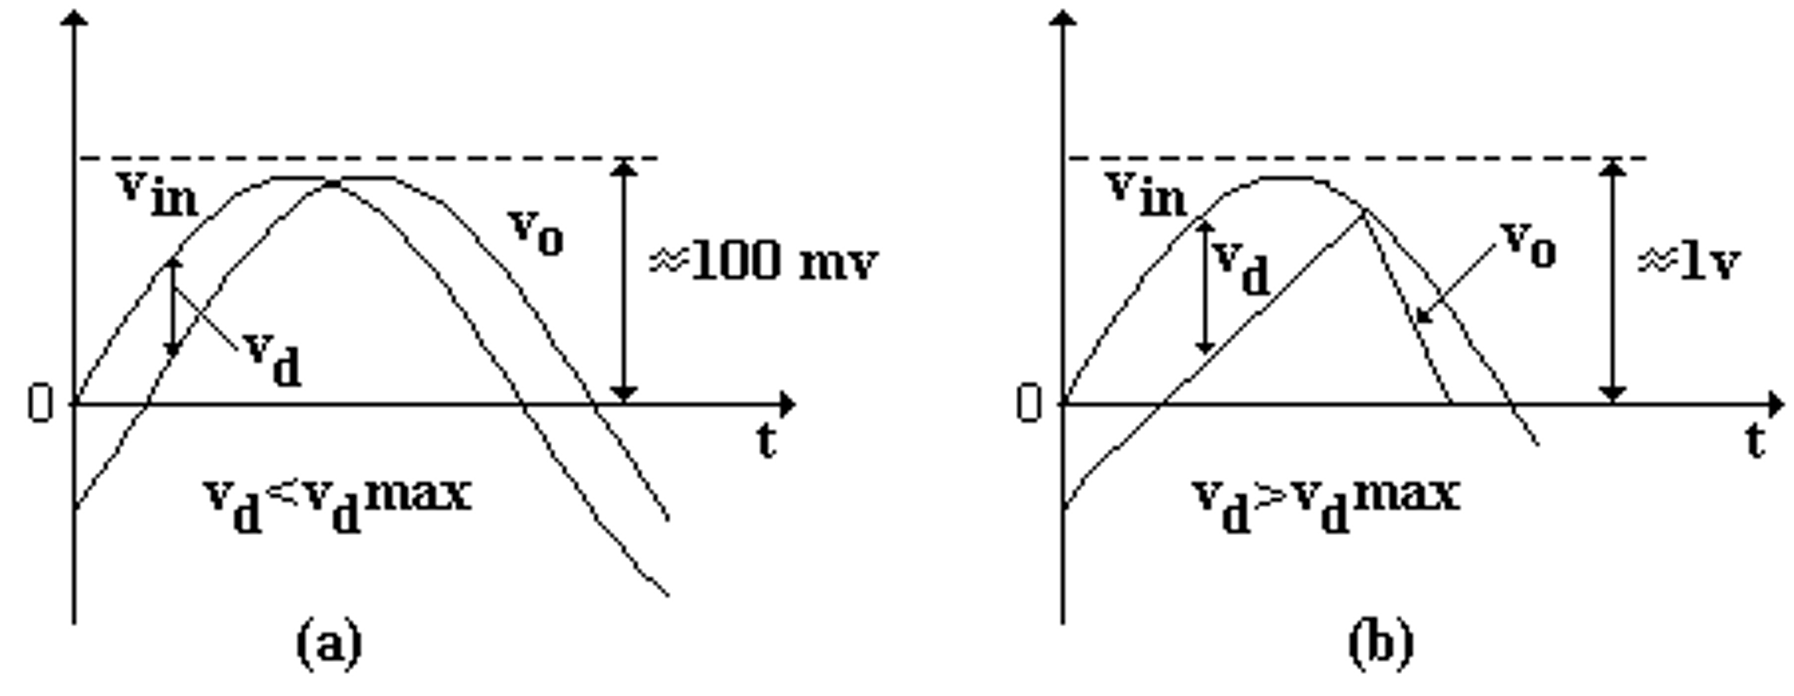
\includegraphics[width=0.5\linewidth]{Imagenes/2.22.png}
    \caption{}
    \label{fig:2.22}
\end{figure}
\noindent Pero si la señal es fuerte (Ej. $v_{in} \ge 1v$) y la velocidad de crecimiento elevada, tal que se llegue a la condición de corriente ($g_m \cdot v_d = I_0$), la tensión de salida varía linealmente ( No puede copiar la entrada, Figura 2.17b). %

\noindent En esta condición la expresión (2.53) queda %

\begin{equation} \tag{2.54}
\frac{dv_0}{dt} \bigg|_{\max} = \frac{I_0}{C_C} = Cte.
\end{equation} %

\noindent La anterior cuantifica el valor máximo que puede tener la velocidad de crecimiento de la tensión de salida, dato que es publicado por el fabricante como \textit{Slew-Rate}. %

\begin{equation} \tag{2.55}
SR = \frac{dv_0}{dt} \bigg|_{\max}
\end{equation} %

\noindent El efecto que produce esta limitación sobre una señal senoidal que ha excedido la condición comentada, se muestra en Figura 2.18. 
\begin{figure}[H]
    \centering
    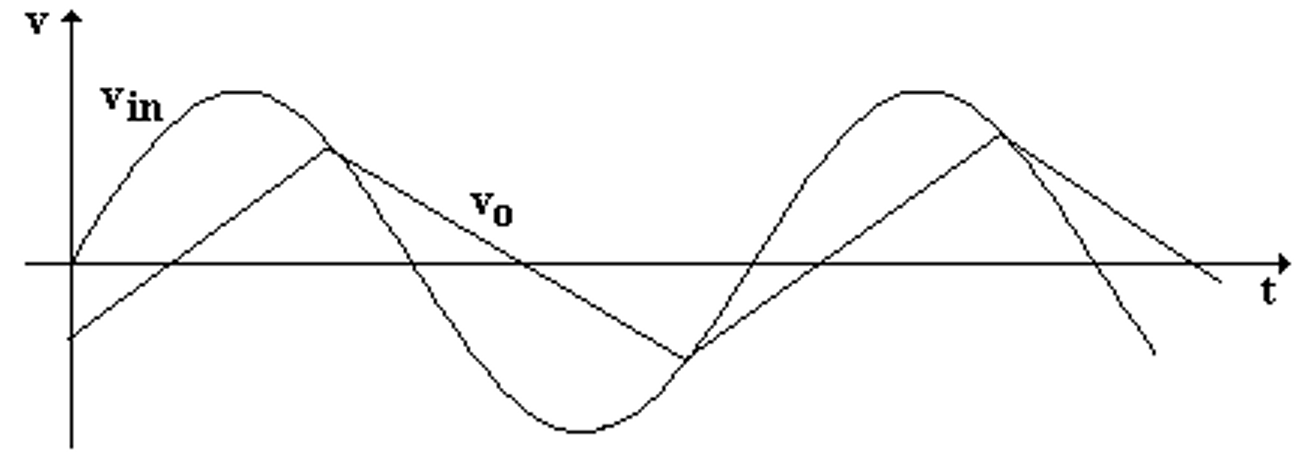
\includegraphics[width=0.5\linewidth]{Imagenes/2.23.png}
    \caption{}
    \label{fig:2.23}
\end{figure}
\subsubsection{Ancho de Banda de Plena Potencia}
\noindent El límite de la velocidad de crecimiento de la tensión de salida, obviamente impone otra cota superior a la respuesta en frecuencia, cuando de grandes excursiones se trata. Este límite se denomina ancho de banda de plena potencia (\textit{Full Power Bandwidth}). Y se define como la máxima frecuencia de una señal senoidal que puede ser reproducida sin distorsión para excursiones de salida elevada (generalmente 10v) se puede demostrar que el ancho de banda de potencia es inversamente proporcional a la amplitud de la señal senoidal.

\vspace{0.3cm}

\noindent En efecto si

\[
v_0 = \hat{v} \cdot \text{sen } \omega \cdot t \quad \rightarrow \quad \frac{dv_0}{dt} = \omega \cdot \hat{v} \cdot \cos \omega \cdot t
\]

\vspace{0.3cm}

\noindent La anteriores máxima para $\cos \omega t = 1$, luego

\begin{equation} \tag{2.56}
\frac{dv_0}{dt} \bigg|_{\max} = SR = \omega_p \cdot \hat{V}_0
\end{equation}

\begin{equation} \tag{2.57}
\omega_{HP} = \frac{SR}{\hat{V}_0}
\end{equation}
\subsection{Problemas unidad 2}
\noindent \textbf{P. 2.1.} Diseñar una configuración no inversora con ganancia $A_{vfi} = 2$ y otra de $A_{vfi} = 200$ ambas con fondo de escala de 5v. Evaluar el error total en continua. Utilizando las siguientes opciones.

\begin{itemize}
    \item[a)] VFA(BIPOLAR) - LM324
    \item[b)] VFA (MOS) – LM6484
\end{itemize}

\noindent \textbf{P. 2.2.} Evaluar el error total para la componente de continua en términos absolutos y relativos a un fondo de escala de 10v, de la tensión de salida del circuito conversor \textit{I-V} del problema P1.6 Utilice las siguientes opciones

\begin{itemize}
    \item[a)] VFA(BIPOLAR) - LM324.
    \item[b)] VFA (FET) - OPA2107
\end{itemize}

\noindent \textbf{P. 2.3.} Analizar el error total propagado a la salida, para la componente de continua en las configuraciones amplificadoras analizadas en P 1.3 y P1.4. Suponga un ajuste perfecto de los valores de las resistencias utilizadas.

\noindent \textbf{P. 2.4.} Diseñar un amplificador diferencial de instrumentación de las siguientes características: Configuración de cuatro AO´s. Rango de excursión de tensión de salida 0-5v con el cero de escala en 2.5v. Ganancia ajustable de 2 a 10 veces. Utilizar el A.O- LM6484. Evaluar el error total a frecuencia cero y verificarlo por simulación en SPICE a $-25^\circ$, $25^\circ$ y $80^\circ$.

\noindent \textbf{P. 2.5} La fórmula de Black, $A_{vf}(s) = A_v(s)/(1-T(s))$, da la expresión de la ganancia de lazo cerrado para un amplificador realimentado y es equivalente a la genérica siguiente $A_{vfi(s)} / (1-(1/T(s)))$. Donde $A_{vfi(s)} = GLC$ (ideal).

\noindent Demuéstrelo para una configuración diferencial simple (fig 1.5), para el conversor I-V del P1.2 y para el amplificador de alterna de Fig 1.7. Suponga al amplificador utilizado con ganancia de modo diferencial con un solo polo $A_{d(S)} = Ad_{(o)} / (1+ s / \omega_1 )$.

\noindent \textbf{P. 2.6.} En el problema P.2.1 el fotodiodo tiene una impedancia interna $r_d = 10 \text{ Megohms}$ y utiliza VFA-LM6484. Dibuje el diagrama de Módulos de GLC, GLA y T. Deduzca el ancho de banda de 3db ($\omega_H$) de la configuración.

\noindent \textbf{P. 2.7} Calcule al ancho de banda de 3db ($\omega_H$) y de 1db, en las configuraciones correspondientes al problema P. 2.4.

\noindent \textbf{P.2.8} El rectificador de precisión del problema P1.12 y 1.13, utiliza el VFA-LM324. Evalúe el ancho de banda de 3db de ambas configuraciones.

\noindent \textbf{P.2.8.} El amplificador de alterna del P.1.5 utiliza el AO-LM324. Dibuje el diagrama de módulos de la respuesta (GLA, GL y GLC).